% -*- latex -*-
%%%%%%%%%%%%%%%%%%%%%%%%%%%%%%%%%%%%%%%%%%%%%%%%%%%%%%%%%%%%%%%%
%%%%
%%%% This TeX file is part of the course
%%%% Introduction to Scientific Programming in C++/Fortran2003
%%%% copyright 2017/8 Victor Eijkhout eijkhout@tacc.utexas.edu
%%%%
%%%% array.tex : basic language elements
%%%%
%%%%%%%%%%%%%%%%%%%%%%%%%%%%%%%%%%%%%%%%%%%%%%%%%%%%%%%%%%%%%%%%

\Level 0 {Static arrays}
\label{sec:staticarray}

An \indextermdef{array} is an indexed data structure, that for each
index stores an integer, floating point number, character,
object,\ldots
In scientific applications, arrays often correspond to vectors and
matrices, potentialy of quite large size. (If you know about
\acfp{FEM}, you know that vectors can have sizes in the millions or beyond.)

To define an array you need to declare its size, and you need to give
it its contents. Those actions don't necessarily have to occur
together. (And the contents can later change, as with any other variable.)
However, 
if you know the array size and contents already before you run your
code, you can create the whole array in one statement. There is more
than one syntax for doing so.
%
\verbatimsnippet{arrayinit}

As you see in this example, if \n{a}~is an array, and \n{i} and
integer, then \n{a[i]} is the i'th element.
\begin{itemize}
\item An array element \n{a[i]} can be used to get the value of an
  array element, or it can occur in the left-hand side of an
  assignment to set the value.
\item The \indextermbus{array}{index} (or
  \indextermbus{array}{subscript}) \n{i} starts numbering at zero.
\item Therefore, if an array has $n$ elements, its last element has
  index~\n{n-1}.
\item If you try to get an array elements outside the bounds of the
  array, your program may give a runtime error, but that does not
  necessarily happen. You could just get some random value.
\item An array does not contain the information about its size: you
  have to store that in variable.
\end{itemize}

\Level 1 {Ranging over an array}
\label{sec:arrayrange}

If you need to consider all the elements in an array, there are two
cases. First:

\begin{block}{Range over elements}
  \label{sl:array-range}
  You can write a \indextermsub{range-based}{for} loop, which
  considers the elements as a collection.
\begin{verbatim}
for ( int i=0; i<N; i++) {
  float e = array[i]; /* something with e */ };
for ( float e : array )
  // statement about element with value e
for ( auto e : array )
  // same, with type deduced by compiler
\end{verbatim}

\snippetwithoutput{rangemax}{array}{rangemax}
\end{block}

(You can spell out \n{for (float e : array)} but \indextermtt{auto} is
quite convenient.)

\begin{block}{Indexing the elements}
  \label{sl:index-range}
  You can write an \indextermsub{indexed}{for} loop, which uses an
  index variable that ranges from the first to the last element.
\begin{verbatim}
for (int i= /* from first to last index */ )
  // statement about index i
\end{verbatim}
\snippetwithoutput{idxmax}{array}{idxmax}
\end{block}

\begin{exercise}
  \label{ex:array-max}
  Find the element with maximum absolute value in an array. Use:
\begin{verbatim}
int numbers[] = {1,-4,2,-6,5};
\end{verbatim}
Which mechanism do you use for traversing the array?

Hint:
\begin{verbatim}
#include <cmath>
..
absx = abs(x);
\end{verbatim}
\end{exercise}

\begin{exercise}
  \label{ex:array-maxidx}
  Find the location of the first negative element in an array.

  Which mechanism do you use?
\end{exercise}

\begin{exercise}
  \label{ex:array-sorted}
  Check whether an array is sorted.
\end{exercise}

\begin{block}{Range over elements by reference}
  \label{sl:array-range-ref}
  Range-based loop indexing makes a copy of the array element. If you
  want to alter the array, use a reference:
\snippetwithoutput{rangescale}{array}{rangescale}
\end{block}

\Level 0 {Vector class for arrays}
\label{sec:stdvector}

Statically allocated arrays are enough for many purposes. However, as
pointed out above, they have some disadvantages. In this section we
will look at one way of dynamically creating arrays: through the STL
\n{vector}.

This takes a new syntax:

\begin{block}{Vector definition}
  \label{sl:vector-def}
\begin{verbatim}
#include <vector>
using std::vector;

vector<type> name;
vector<type> name(size);
vector<type> name(size,value);
\end{verbatim}
where
\begin{itemize}
\item \n{vector} is a keyword,
\item \n{type} (in angle brackets) is any elementary type or class
  name,
\item \n{name} is up to you, and
\item \n{size} is the (initial size of the array). This is an integer,
  or more precisely, a \n{size_t} parameter.
\item \n{value} is the uniform initial value of all elements.
\end{itemize}
\end{block}

\begin{block}{Vector elements}
  \label{sl:vectorsub}
  In a number of ways, vector behaves like an array:
\begin{verbatim}
vector<double> x(5, 0.1 );
x[1] = 3.14;
cout << x[2];
\end{verbatim}
\end{block}

\begin{block}{Ranging over a vector}
  \label{sl:vector-range}
\begin{verbatim}
for ( auto e : my_vector)
  cout << e;
\end{verbatim}
Note that \n{e} is a copy of the array element:
\snippetwithoutput{vectorrangecopy}{array}{vectorrangecopy}
\end{block}

\begin{block}{Ranging over a vector by reference}
  \label{sl:vector-range-ref}
To set array elements, make \n{e} a reference:
\begin{verbatim}
for ( auto &e : my_vector)
  e = ....
\end{verbatim}
\snippetwithoutput{vectorrangeref}{array}{vectorrangeref}
\end{block}

\begin{block}{Vector initialization}
  \label{sl:vector-init}
  You can initialize a vector with much the same syntax as an array:
\begin{verbatim}
vector<int> odd_array{1,3,5,7,9};
vector<int> even_array = {0,2,4,6,8};
\end{verbatim}
(This syntax requires compilation with the \n{-std=c++11}\index{C++11}
option.)
\end{block}

\begin{block}{Vector initialization'}
  \label{sl:vector-initconst}
  There is a syntax for initializing a vector with a constant:
\begin{verbatim}
vector<float> x(25,3.15);
\end{verbatim}
which gives a vector of size~25, with all elements initialized to~3.15.
\end{block}

\begin{block}{Vector copy}
  \label{sl:vectorcopy}
  Vectors can be copied just like other datatypes:
  \snippetwithoutput{vectorcopy}{array}{vectorcopy}
\end{block}

\Level 1 {Vector methods}

A \n{vector} is an object. Let's take a look at some of the methods
that are defined for it.

First of all, there is a way of accessing vector elements through the
\indextermttdef{at} method. It has the big advantage that it does
\indexterm{bounds checking}.
\begin{block}{Vector indexing}
  \label{sl:vector-index}
  Your choice:  fast but unsafe, or slower but safe
\begin{verbatim}
vector<double> x(5);
x[5] = 1.; // will probably work
x.at(5) = 1.; // runtime error!
\end{verbatim}
\end{block}

Safer, but also slower; see below.

The method \n{size} gives the size of the vector:
\begin{verbatim}
vector<char> words(37);
cout << words.size(); // will print 37
\end{verbatim}
The existence of this method means that you don't have to remember the
size of a vector: it has that information internally.

\begin{advanced}
  The vector class is a template class: the type that it uses (int,
  float) is not predetermined, but you can make a vector object out of
  whatever type you like.
\end{advanced}

\begin{slide}{Vector methods}
  \label{sl:vector-method}
  \begin{itemize}
  \item Get elements with \n{ar[3]} (zero-based indexing).\\
    (for C programmers: this is not dereferencing, this uses an
    operator method)
  \item Get elements, including bound checking, with \n{ar.at(3)}.
  \item Size: \n{ar.size()}.
  \item Other functions: \n{front}, \n{back}.
  \end{itemize}
\end{slide}

\Level 1 {Vectors are dynamic}
\label{sec:stdvector-dynamic}

There is an important difference between vectors and arrays: a vector
can be grown or shrunk after its creation.
Use the \n{push_back} method to add elements at the end:

\begin{block}{Dynamic extension}
  \label{sl:vector-dynamic}
\begin{verbatim}
vector<int> array(5);
array.push_back(35);
cout << array.size(); // is now 6 !
\end{verbatim}
also \n{pop_back}, \n{insert}, \n{erase}.\\
Flexibility comes with a price.
\end{block}

This is not a good way of creating arrays: if you know the size, it is
better to reserve the vector at the correct size.

Other methods that change the size: \n{insert}, \n{erase}.

\Level 1 {Vector assignment}

The limitation that you couldn't create an array in an object still
holds:

\begin{block}{Can you make a class around a vector?}
  \label{sl:class-with-vector}
  Vector needs to be created with the object:
\begin{verbatim}
class witharray {
private:
  vector<int> the_array( ???? );
public:
  witharray( int n ) {
    thearray( ???? n ???? );
  }
}
\end{verbatim}
\end{block}

\begin{block}{Create and assign}
  \label{sl:class-has-vector}
  The following mechanism works:
\begin{verbatim}
class witharray {
private:
  vector<int> the_array;
public:
  witharray( int n ) {
    thearray = vector<int>(n);
  }
}
\end{verbatim}
\end{block}

You could read this as
\begin{itemize}
\item \n{vector<int> the_array} declares a int-vector variable, and
\item \n{thearray = vector<int>(n)} assigns an array to it.
\end{itemize}
However, 
technically, it actually does the following:
\begin{itemize}
\item The class object initially has a zero-size vector;
\item the expression \n{vector<int>(n)} creates an anonymous vector
  of size~\n{n};
\item which is then assigned to the variable \n{the_array},
\item so now you have an object with a vector of size~\n{n} internally.
\end{itemize}

\Level 1 {Vectors and functions}

\Level 2 {Vector as function return}

\begin{block}{Vector as function return}
  \label{sl:vector-return}
  You can have a vector as return type of a function:
  %
  \snippetwithoutput{vectorreturn}{array}{vectorreturn}
\end{block}

\Level 2 {Pass vector to function}

\begin{block}{Vector as function argument}
  \label{sl:vector-arg}
  You can pass a vector to a function:
\begin{verbatim}
void print0( vector<double> v ) {
  cout << v[0] << endl;
};
\end{verbatim}
Vectors, like any argument, are passed by value, so the vector is
actually copied into the function.
\end{block}

\begin{block}{Vector pass by value example}
  \label{sl:vector-arg-ex}
  \snippetwithoutput{vectorpassval}{array}{vectorpassnot}  
\end{block}

\begin{block}{Vector pass by reference}
  \label{sl:vector-arg-ref}
  If you want to alter the vector, you have to pass by reference:
  %
  \snippetwithoutput{vectorpassref}{array}{vectorpassref}  
\end{block}

\begin{exercise}
  \label{ex:vec-rand-sort}
  Write functions \n{random_vector} and \n{sort} to make the following
  main program work:
\begin{verbatim}
int length = 10;
vector<float> values = random_floats(length);
sort(values);
\end{verbatim}
  (This creates a vector of random values of a specified length, and
then sorts it.)
\end{exercise}

\Level 1 {Dynamic size of vector}

Writing

\begin{block}{Dynamic size extending}
  \label{sl:vector-extend}
\begin{verbatim}
vector<int> iarray;
\end{verbatim}
creates a vector of size zero. You can then
\begin{verbatim}
iarray.push_back(5);
iarray.push_back(32);
iarray.push_back(4);
\end{verbatim}
\end{block}

to add elements to the vector, dynamically resizing it. Since this
requires operating system actions, it will probably be inefficient.

\Level 1 {Timing}

Different ways of acessing a vector can have drastically different
timing cost.

\begin{block}{Vector extension}
  \label{sl:vect-extend-code}
  You can push elements into a vector:
  \verbatimsnippet{vectorflex}

  If you allocate the vector statically, you can assign with \n{at}:
  \verbatimsnippet{vectorat}
\end{block}

\begin{block}{Vector extension}
  \label{sl:vect-extend-code2}
  With subscript:
  \verbatimsnippet{vectorsub}

  You can also use \n{new} to allocate:
  \verbatimsnippet{vectornew}
\end{block}

Timings are partly predictable, partly surprising:
\begin{block}{Timing}
  \label{sl:vector-extend-time}
\begin{verbatim}
  Flexible time: 2.445
  Static at time: 1.177
  Static assign time: 0.334
  Static assign time to new: 0.467
\end{verbatim}
\end{block}

The increased time for \n{new} is a mystery.

So do you use \n{at} for safety or \n{[]} for speed? Well, you could
use \n{at} during development of the code, and insert
\begin{verbatim}
#define at(x) operator[](x)
\end{verbatim}
for production.

\Level 0 {Use of \texttt{new}}

\prerequisite{\ref{sec:arraypointer}}

There is a dynamic allocation mechanism that is much inspired by
memory management in~C. Don't use this as your first choice.

Use of \indextermtt{new} uses the 
equivalence of array and reference.
%
\verbatimsnippet{arrayfromfunc}

Since this is not scoped, you have to free the memory yourself:
%
\verbatimsnippet{arrayinclass}

Notice how you have to remember the array length yourself? This is all
much easier by using a \n{std::vector}. See
\url{http://www.cplusplus.com/articles/37Mf92yv/}.

The \n{new} mechanism is a cleaner variant of \indextermtt{malloc},
which was the dynamic allocation mechanism in~C. It is still
available, but should not be used.

\Level 0 {Wrapping a vector in an object}

You may want to a create objects that contain a vector, for instance
because you want to add some methods.
%
\verbatimsnippet{printablevector}

Unfortunately this means you may have to recreate some methods:
%
\verbatimsnippet{vectorinheritat}

\Level 0 {Old-style arrays}

Static arrays are really an abuse of the equivalence of arrays and
addresses of the C programming language. This appears for instance in
parameter passing mechanisms.

\Level 1 {Arrays and subprograms}

Arrays can be passed to a subprogram, but the bound is unknown there.
%
\verbatimsnippet{arraypass}
%
\begin{exercise}
  Rewrite the above exercises where the sorting tester or the maximum
  finder is in a subprogram.
\end{exercise}

Subprograms can alter array elements. This was not possible with
scalar arguments.

\Level 0 {Multi-dimensional cases}

\Level 1 {Matrix as vector of vectors}

\begin{block}{Multi-dimensional vectors}
  \label{sl:multi-vector}
  Multi-dimensional is harder with vectors:
\begin{verbatim}
vector<float> row(20);
vector<vector<float>> rows(10,row);
\end{verbatim}
Vector of vectors.
\end{block}

This is not contiguous.

\Level 1 {Matrix class based on vector}

You can make a `pretend' matrix by storing a long enough \n{vector} in
an object:
%
\verbatimsnippet{matrixclass}

The syntax for \n{set} and \n{get} can be improved.
\begin{exercise}
  Write a method \n{element} of type \n{double&}, so that you can write
\begin{verbatim}
A.element(2,3) = 7.24;
\end{verbatim}
\end{exercise}

\Level 1 {A matrix class}

\begin{block}{Matrix class}
  \label{sl:matrix-class}
  \verbatimsnippet{matrixclassdef}
\end{block}

\begin{block}{Matrix class'}
  \label{sl:matrix-class-cont}
  Better idea:
\begin{verbatim}
  elements = vector<double>(rows*cols);
  ...
  void get(int i,int j) {
    return elements.at(i*cols+j);
  }
\end{verbatim}
\end{block}


\begin{exercise}
  \label{ex:matrix-methods}
  Add methods such as \n{transpose}, \n{scale} to your matrix class.

  Implement matrix-matrix multiplication.
\end{exercise}

\Level 0 {Multi-dimensional arrays}

Multi-dimensional arrays can be declared and used with a simple extension of
the prior syntax:
\begin{verbatim}
float matrix[15][25];

for (int i=0; i<15; i++)
  for (int j=0; j<25; j++)
    // something with matrix[i][j]
\end{verbatim}

Passing a multi-dimensional array to a function, only the first
dimension can be left unspecified:
%
\verbatimsnippet{arraypass2d}

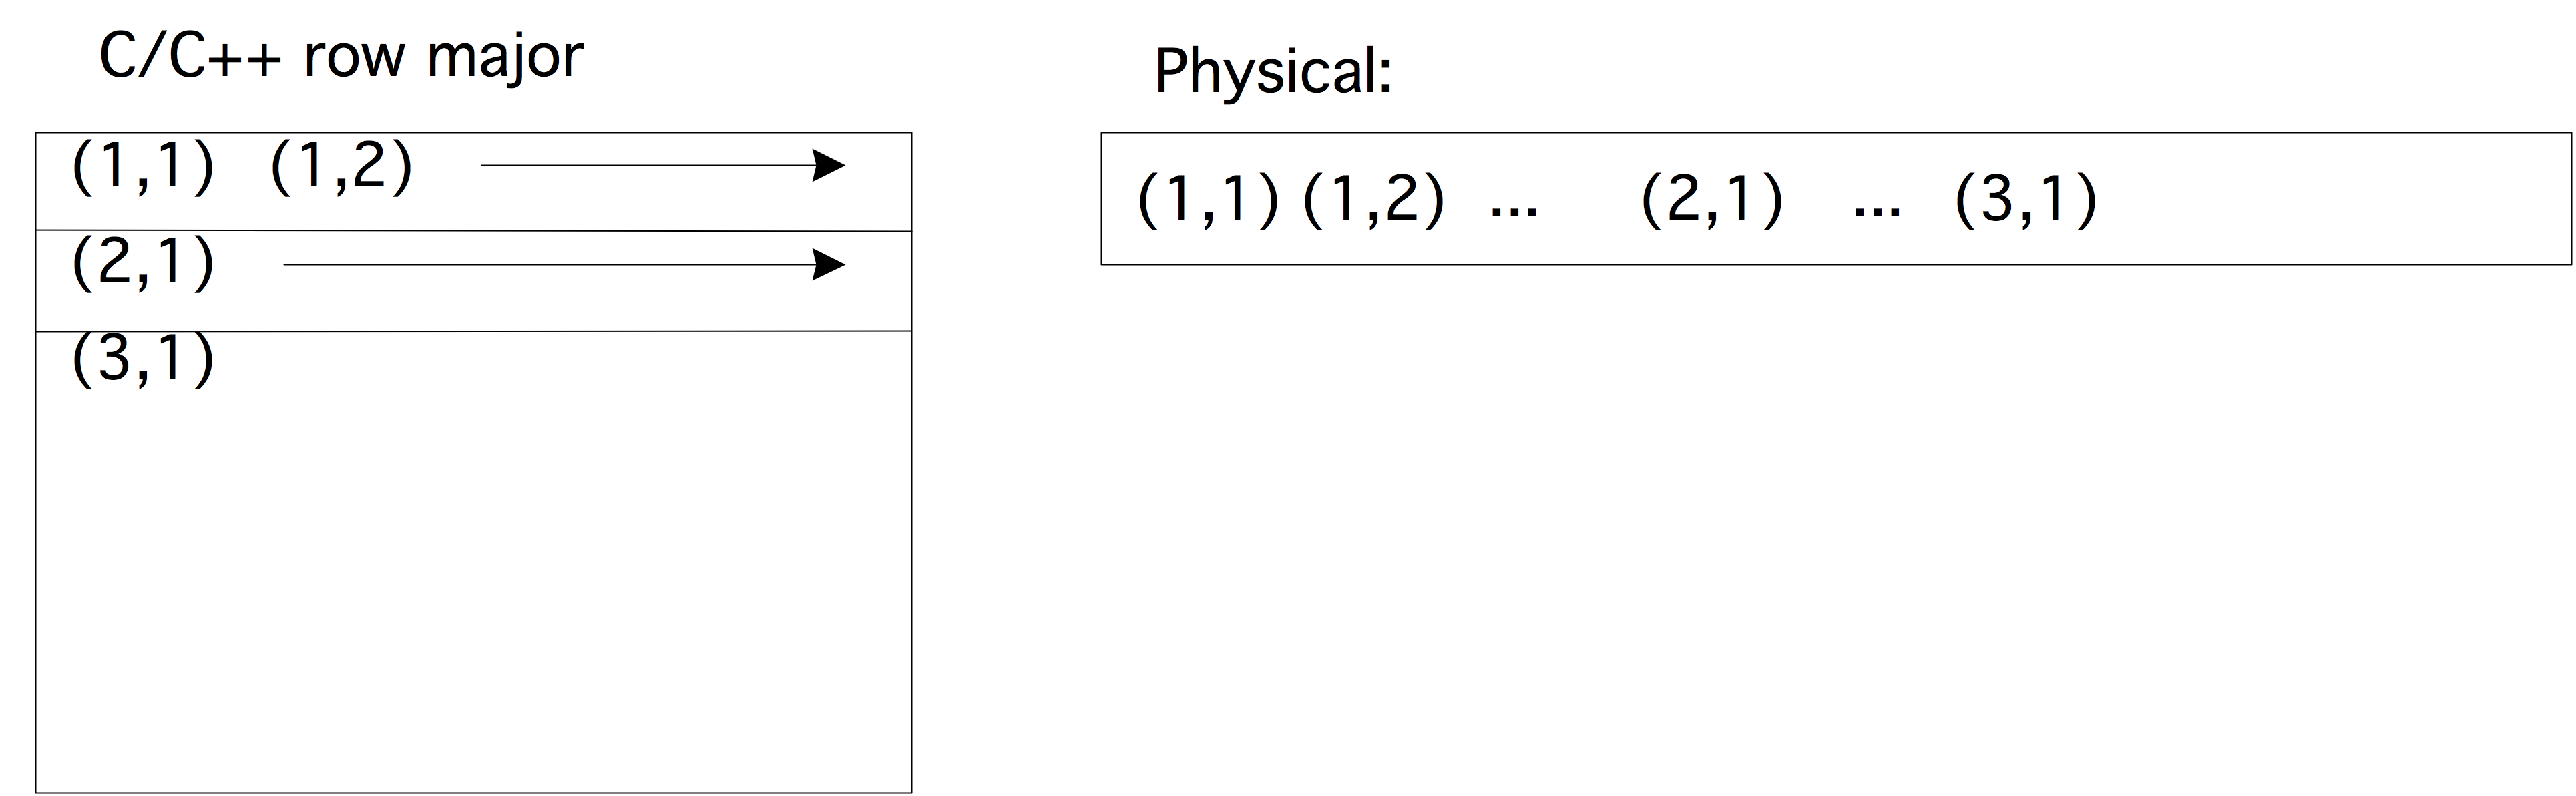
\includegraphics[scale=.1]{arrayc}

\Level 1 {Memory layout}

Puzzling aspects of arrays, such as which dimensions need to be
specified and which not in a function call, can be understood by
considering how arrays are stored in memory.
The question then is how a two-dimensional (or higher dimensional)
array is mapped to memory, which is linear.
\begin{itemize}
\item A one-dimensional array is stored in contiguous memory.
\item A two-dimensional array is also stored contiguously, with first
  the first row, then the second, et cetera.
\item Higher dimensional arrays continue this notion, with contiguous
  blocks of the highest so many dimensions.
\end{itemize}

As a result of this, indexing beyond the end of a row, brings you to the
start of the next row:
%
\verbatimsnippet{arraywrap}

We can now also understand how arrays are passed to functions:
\begin{itemize}
\item The only information passed to a function is the address of the
  first element of the array;
\item In order to be able to find location of the second row (and
  third, et cetera), the subprogram needs to know the length of each
  row.
\item In the higher dimensional case, the subprogram needs to know the
  size of all dimensions except for the first one.
\end{itemize}

\Level 0 {Dynamically allocated arrays}
\label{sec:arraynew}

(To properly understand this section, you also need to read
section~\ref{sec:arraypointer}.)

A declaration 
\begin{verbatim}
float ar[500];
\end{verbatim}
is local to the scope it is in. This has some problems:
\begin{itemize}
\item Allocated on the \indexterm{stack}; may lead to stack overflow.
\item Can not be used as a class member:
\begin{verbatim}
class thing {
private:
  double array[ ???? ];
public:
  thing(int n) {
    array[ n ] ???? this does not work
  }
}
\end{verbatim}
\item Can not be returned from subprogram:
\begin{verbatim}
void make_array( double array[],int n ) {
  double array[n] ???? does not work
}
int main() {
  ....
  make_array(array,100);
}
\end{verbatim}
\end{itemize}

We will now look at several strategies for dynamically creating arrays.

\Level 0 {Exercises}

\begin{exercise}
  Program \indexterm{bubble sort}: go through the array comparing
  successive pairs of elements, and swapping them if the second is
  smaller than the first. After you have gone through the array, the
  largest element is in the last location. Go through the array again,
  swapping elements, which puts the second largest element in the
  one-before-last location. Et cetera.
\end{exercise}

\begin{block}{Pascal's triangle}
  \label{sl:pascal-def}
  \small
  Pascal's triangle contains binomial coefficients:
\begin{verbatim}
Row    1:                     1
Row    2:                   1   1
Row    3:                 1   2   1
Row    4:               1   3   3   1
Row    5:             1   4   6   4   1
Row    6:           1   5  10  10   5   1
Row    7:         1   6  15  20  15   6   1
Row    8:       1   7  21  35  35  21   7   1
Row    9:     1   8  28  56  70  56  28   8   1
Row   10:   1   9  36  84 126 126  84  36   9   1
\end{verbatim}
where \[ p_{rc} = \begin{pmatrix} r\\c \end{pmatrix} = \frac{r!}{c!(r-c)! }. \]
The coefficients can easily be computed from the recurrence
\[ p_{rc} = 
\begin{cases}
  1&c\equiv 1\vee c\equiv r\\
  p_{r-1,c-1}+p_{r-1,c}
\end{cases}
\]
\end{block}

\begin{exercise}
  \label{ex:pascal-ex}
  \small
  \begin{itemize}
  \item 
    Write a class \n{pascal} so that \n{pascal(n)} is the object
    containing $n$~rows of the above coefficients. Write a method
    \n{get(i,j)} that returns the $(i,j)$ coefficient.
  \item
    Write a method \n{print} that prints the above display.
  \item
    Write a method \n{print(int m)} that prints a star if the
    coefficient modulo~$m$ is nonzero, and a space otherwise.
\begin{verbatim}
          *
         * *
        *   *
       * * * *
      *       *
     * *     * *
    *   *   *   *
   * * * * * * * *
  *               *
 * *             * *
\end{verbatim}
  \item
    The object needs to have an array internally. The easiest solution
    is to make an array of size $n\times n$.

    Bonus: when you have that code working, optimize your code to use
    precisely enough space for the coefficients.
  \end{itemize}
\end{exercise}

\begin{exercise}
  A knight on the chess board moves by going two steps horizontally or
  vertically, and one step either way in the orthogonal
  direction. Given a starting position, find a sequence of moves that
  brings a knight back to its starting position. Are there starting
  positions for which such a cycle doesn't exist?
\end{exercise}

\begin{exercise}
  Put eight queens on a chessboard so that none threatens any other.
\end{exercise}

\begin{exercise}
  From the `Keeping it REAL' book, exercise 3.6 about Markov chains.
\end{exercise}
